\chapter{Testovanie}
\label{kap:testovanie}
Študenti mali možnosť využívať časť novej funkcionality už od začiatku výučby predmetu Logika pre informatikov v letnom semestri akademického roka 2025/2026. Išlo najmä o grafové editory, maticový editor a databázový editor, ktoré boli v tom čase už z veľkej časti dokončené. Ostatné nástroje sme postupne pridávali v priebehu semestra. Predvoleným editorom bol však väčšinou množinový (textový) pohľad. Na podrobnejšie otestovanie nových editorov sme sa preto rozhodli na jednom z posledných cvičení študentom pri vhodných interpretáciách naopak predvoliť orientovaný graf a editor interpretácií funkcií rozborom prípadov. Tie niekedy slúžili len na vizualizáciu, inokedy bolo pomocu nich potrebné aj upravovať samotnú interpretáciu. Medzi jednotlivými pohľadmi mohli študenti však aj naďalej ľubovoľne prepínať. Príklad jednej štruktúry z cvičenia je na obrázku \ref{obr:test-struct}.\footnote{Pre prehľadnosť obrázka boli odstránené interpretácie niektorých mimologických symbolov.}

Po vypracovaní cvičenia mali študenti možnosť vyplniť krátky dotazník zameraný na získanie spätnej väzby k použiteľnosti pridaných editorov (dotazník možno vidieť na obrázku \ref{obr:sus-dotaznik}). Jeho hlavná časť bola zameraná na ohodnotenie použiteľnosti navrhnutých riešení prostredníctvom 10 výrokov prevzatých zo štandardného dotazníka System Usability Scale (SUS) \cite{sus}. Pri každom výroku študenti vyjadrovali mieru súhlasu na škále od 1 (rozhodne nesúhlasím) do 5 (rozhodne súhlasím). Na základe odpovedí sa následne vypočítava skóre v rozsahu od 0 do 100, pričom vyššia hodnota znamená lepšiu použiteľnosť.

Dotazník celkovo vyplnilo 49 študentov. Priemerné skóre nám vyšlo 63, čo naznačuje, že študenti pri používaní nových riešení identifikovali určité nedostatky, na ktorých by bolo vhodné ešte zapracovať. Histogram na obrázku \ref{fig:histogram-skore} zobrazuje početnosť jednotlivých SUS skóre.

\begin{figure}
    \centering
    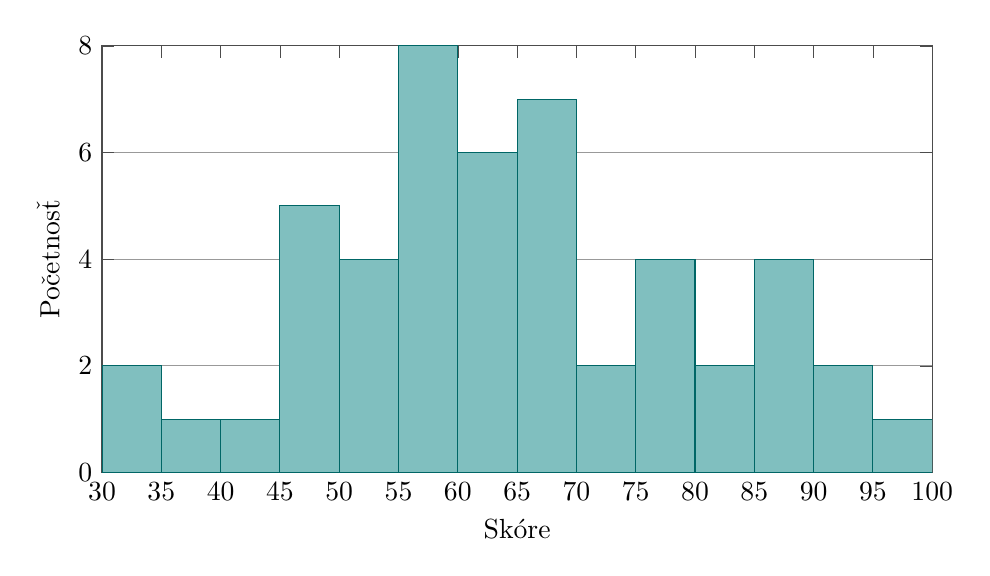
\begin{tikzpicture}
        \begin{axis}[
                width=\textwidth,
                height=7cm,
                xmin=30, xmax=100,
                ymin=0, ymax=8,
                xtick distance=5,
                ytick distance=2,
                ymajorgrids=true,
                grid style={black!40},
                axis line style={black!70},
                tick style={black!70},
                xlabel={Skóre},
                ylabel={Početnosť},
                area style,
                axis on top=false,
            ]
            \addplot+[
                ybar interval,
                fill=teal!50,
                draw=teal!80!black,
            ] plot coordinates {
                    (30,2) (35,1) (40,1) (45,5) (50,4)
                    (55,8) (60,6) (65,7) (70,2) (75,4)
                    (80,2) (85,4) (90,2) (95,1) (100,0)
                };
        \end{axis}
    \end{tikzpicture}
    \caption{Histogram jednotlivých SUS skóre z testovania použiteľnosti.}
    \label{fig:histogram-skore}
\end{figure}

Najhoršie dopadla otázka zameraná na to, či si študent myslí, že by sa musel naučiť veľa vecí, kým by vedel s novými editormi začať pracovať. S výrokom spolu skôr súhlasilo 11 študentov, 23 skôr nesúhlasilo a 15 odpovedalo neutrálne. Naopak najlepší výsledok sme zaznamenali pri otázke, či podľa študenta boli jednotlivé funkcie nových editorov dobre integrované. S výrokom skôr súhlasilo 33 študentov, 4 skôr nesúhlasili a 12 odpovedalo neutrálne. Podobné výsledky sme zaznamenali aj pri ďalších otázkach tohto typu. Rozdiel si vysvetľujeme tak, že študenti nemali často problém s tým, ako jednotlivé editory fungujú, ale skôr s pochopením alebo objavením ich jednotlivých možností. Tento problém sme sa snažili ďalej zmierniť pridaním lepších vysvetliviek k~ovládacím prvkom a zrozumiteľnejšou komunikáciou niektorých stavov editorov.

Na konci dotazníka mohli študenti uviesť konkrétne problémy, na ktoré narazili, ako aj prípadné návrhy na ich zlepšenie. Často sa opakovala pripomienka na nadmerné množstvo vnorených rolovateľných prvkov v rámci celej aplikácie Logického pracovného zošita. Je to spôsobené najmä tým, že vertikálne možno rolovať nie len celý hárok, ale aj obsah vložených aplikácií. Grafové editory k tomuto navyše pridali ďalší element reagujúci na rolovanie, keďže pri umiestení kurzora nad zobrazenie grafu je možné jeho obsah zväčšovať alebo zmenšovať. Pri hľadaní vhodného riešenia nás oslovila spätná väzba jedného študenta. V nej navrhol, aby bolo rolovanie v grafoch možné len v~prípade, ak je zároveň stlačené pridružené tlačidlo (napr. \texttt{Ctrl}), podobne ako je to pri zobrazeniach máp Google vložených do iných webových stránok. Všetky grafové pohľady sme doplnili o takéto správanie.

Niektorí študenti mali problém aj s tým, že pri pridávaní viacerých nových prvkov domény sa im prislúchajúce vrcholy v zobrazení orientovaného grafu vzájomne prekrývali, čo pôsobilo mätúco. Tento problém sme vyriešili náhodným rozmiestnením nových vrcholov.

Na podnet jedného študenta sme sa tiež rozhodli upraviť editor interpretácií funkcií rozborom prípadov tak, aby pri určovaní podmienky bolo možné zadávať viacero prvkov, nielen jeden konkrétny. Vďaka tomu je tvorba podmienok v určitých situáciách jednoduchšia, keďže nie je potrebné definovať samostatný prípad pre každú hodnotu podmienky. Novú verziu editora interpretácií funkcií rozborom prípadov možno vidieť na obrázku \ref{obr:reworked-case-tree}. Editor sme navyše vylepšili aj pridaním správy „all cases for $\langle\textit{argument funkcie}\rangle$ covered“, ktorá značí, že hodnota funkcie je už definovaná pre všetky možné hodnoty daného argumentu. Ak však ešte nie je, používateľ teraz môže umiestnením kurzora nad text „is any other“ vo všeobecnej podmienke pre daný argument zistiť, o ktoré prvky domény sa jedná.

\begin{figure}[tbhp]
    \centerline{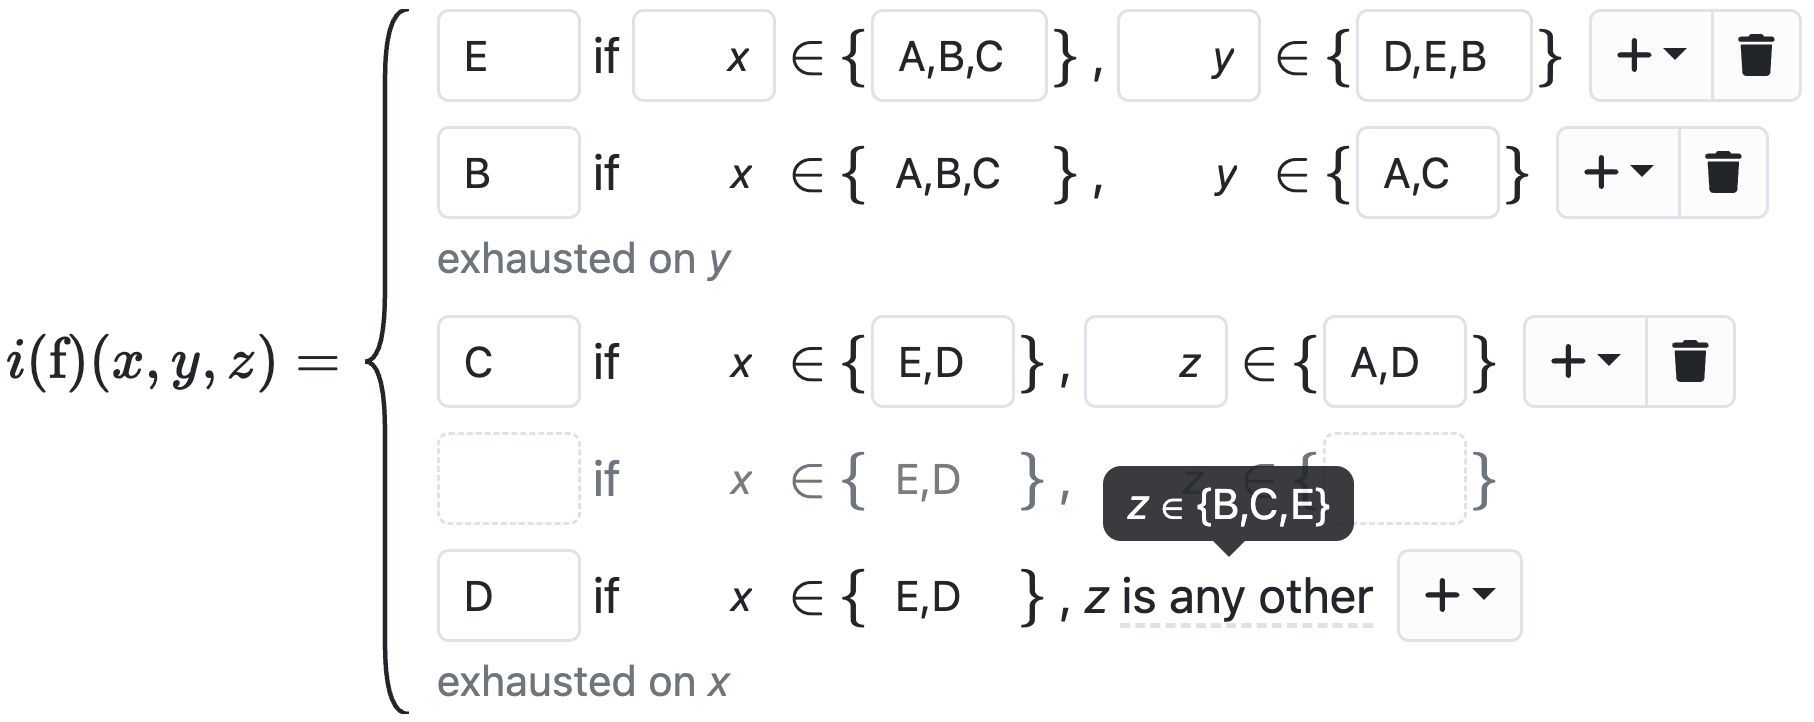
\includegraphics[width=0.92\textwidth]{images/reworked-case-tree.png}}
    %popis obrazku
    \caption[Nová verzia editora interpretácií funkcií rozborom prípadov.]{Nová verzia editora interpretácií funkcií rozborom prípadov.}
    %id obrazku, pomocou ktoreho sa budeme na obrazok odvolavat
    \label{obr:reworked-case-tree}
\end{figure}

%Veríme, že spomínané zmeny pomohli s problémami, ktoré študenti pri používaní nových editorov odhalili. Výrazne nám pri hľadaní vhodných riešení pomohla aj spätná väzba študentov. Cieľom pri ďalšom testovaní aplikácie by určite bolo dosiahnutie lepšieho SUS skóre. Na ďalšie testovanie aplikácie už však na predmete nie je priestor.

Veríme, že spomínané zmeny pomohli odstrániť problémy, ktoré študenti odhalili pri používaní nových editorov. Cieľom ďalšieho testovania aplikácie by určite bolo dosiahnuť lepšie SUS skóre, no v rámci predmetu už naň nie je priestor. Nové vylepšenia a ich prípadné testovanie preto ponechávame na budúci vývoj aplikácie.


% \begin{figure}
%     \centerline{
\includegraphics[width=0.98\textwidth]{\imgdir/test-structure-whole.png}}
%     %popis obrazku
%     \caption[Štruktúra z cvičenia zameraného na testovanie alternatívnych editorov.]{Štruktúra z cvičenia zameraného na testovanie alternatívnych editorov.}
%     %id obrazku, pomocou ktoreho sa budeme na obrazok odvolavat
%     \label{obr:test-struct}
% \end{figure}

%\begin{figure}[h]
%    \centering
%    \begin{subfigure}{0.49\textwidth}
%        \centering
%        
\includegraphics[width=\linewidth]{\imgdir/test-structure-2.png}
%        \caption{Pôvodná verzia}
%    \end{subfigure}
%    \hfill
%    \begin{subfigure}{0.49\textwidth}
%        \centering
%        
\includegraphics[width=\linewidth]{\imgdir/test-structure-1.png}
%        \caption{Nová verzia}
%    \end{subfigure}
%    \caption{Porovnanie pôvodného a nového rozhrania Henkinovej-Hintikkovej hry.}
%    \label{obr:test-structs}
%\end{figure}